\section{ReiserFS}
\subsection{Introducción}
\begin{frame}{Introducción}
  \begin{itemize}
    \item Sistema de propósito general.
    \item Muy bueno en tratamiento de ficheros pequeños.
    \item Primero sistema de ficheros con Journaling incluido en el kernel de Linux.
    \item Es el sistema de ficheros por defecto en varias distribuciones.
    \item Actualmente Namesys ha dejado el desarrollo de ReiserFS para centrarse en su sucesor Reiser4.
  \end{itemize}
\end{frame}

\subsection{Características}
\begin{frame}{Características}
  \begin{itemize}
    \item Journaling
    \item ACLs
    \item Permisos POSIX
    \item Tamaño máximo: 16TB
    \item Tamaño máximo de fichero: 16TB
    \item Máximo de caracteres de nombre de fichero: 256B
    \item Máximo número de ficheros: 4.294.967.293
  \end{itemize}
\end{frame}

\subsection{Estructura}
\begin{frame}{Estructura}
  \begin{itemize}
    \item Al principio de la partición nos encontramos el sector de arranque.
    \item Justo después se encuentra el superblock.
    \item Para el resto de la partición se van alternando mapas de bits de bloques y bloques de datos.
    \item Cada mapa de bits de bloques se refiere al bloque de datos que queda después de el y nos da información sobre los bloques libres  y ocupados.
    \item Cada bloque de datos contiene los datos e inodos.
  \end{itemize}
\end{frame}

\begin{frame}{Estructura}
  \begin{center}
    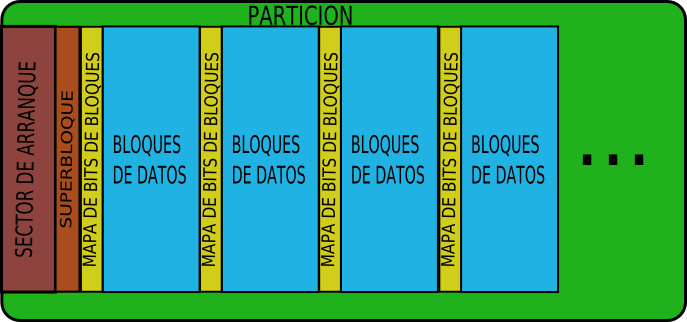
\includegraphics[height=5.5cm]{imgs/reiserfs_struct.png}
  \end{center}
\end{frame}

\begin{frame}{Ficheros}
  \begin{itemize}
    \item Existen 4 tipos de objetos: stat, directorios, directos e indirectos.
    \item Todos los ficheros en reiser tienen asociado un objeto stat, el cual almacena información de permisos.
    \item Los directorios a su vez tienen asociados uno o más objetos del tipo directorio, tantos como hagan falta para almacenar todas las entradas del directorio.
    \item Los ficheros regulares, si son pequeños se asocian a un objeto directo que almacena los datos, si son grandes se asocia a uno o varios objetos indirectos que contienen punteros a bloques de datos.
  \end{itemize}
\end{frame}

\begin{frame}{Ficheros}
  \begin{center}
    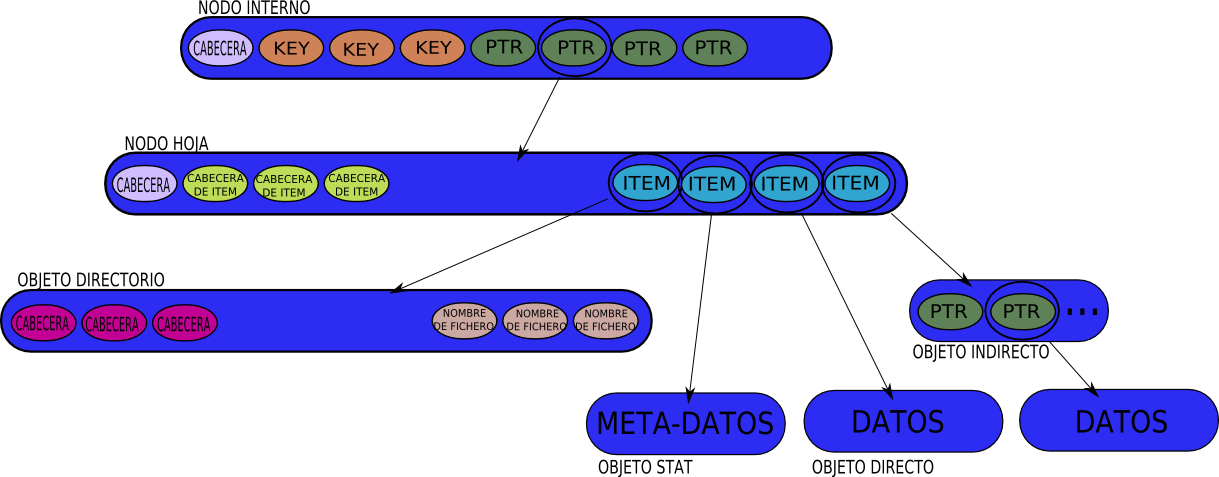
\includegraphics[height=4.5cm]{imgs/reiserfs_files.png}
  \end{center}
\end{frame}
